\section{Introduction to $p$-$n$ Junction}\label{sec:sec001}
A $p$-$n$ junction is formed when a $p$-type semiconductor is and an $n$-type semiconductor are in contact.
Understanding this basic configuration creates a foundation for much of modern electronic
applications and other semiconductor devices. These $p$-$n$ junctions are fundamental to a variety of functions
such as rectification, amplification, switching, and other applications which can be achieved by varying parameters 
of the junction. 

\section{$p$-$n$ Junction in Equilibrium}\label{sec:sec002}
In the most basic sense, one can consider a $p$-$n$ junction under thermodynamic equilibrium with 
constant doping concentrations. The band diagrams of the $p$ and $n$-type materials before they are brought
into contact with each other are pictured in  fig. \ref{fig:fig01}. 

\begin{figure}[h!]\label{fig:fig01}
    \centering
    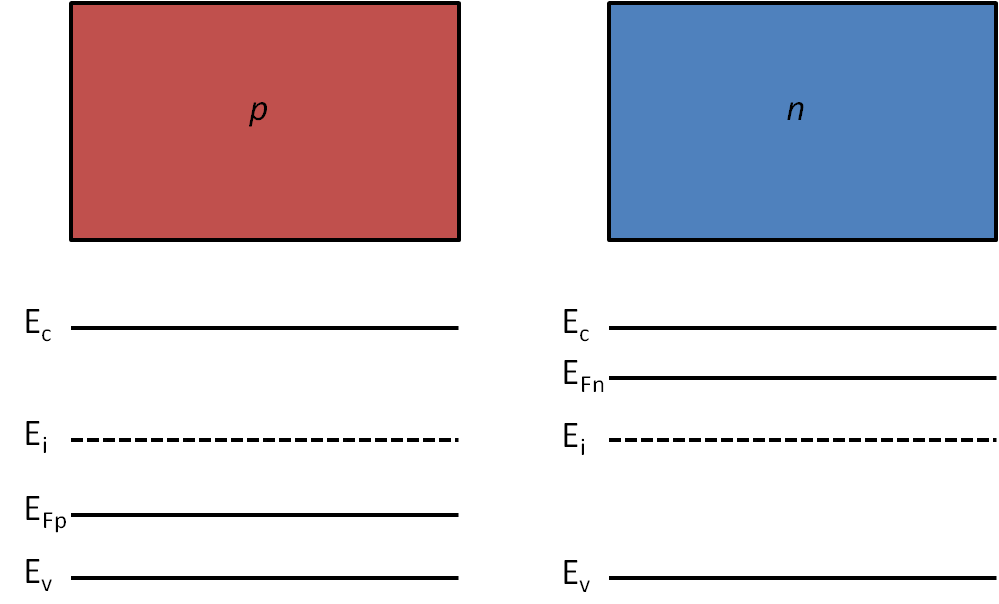
\includegraphics[height=5cm,width=8.5cm]{figs/unbiased_pn_junction_bands}
    \caption{Energy band diagram of the $p$ and $n$-type regions taken separately.}
\end{figure}

Once the regions of differing types are brought into contact with each other the band diagram is as
pictured in fig. \ref{fig:fig02}. 

\begin{figure}[h!]\label{fig:fig02}
    \centering
    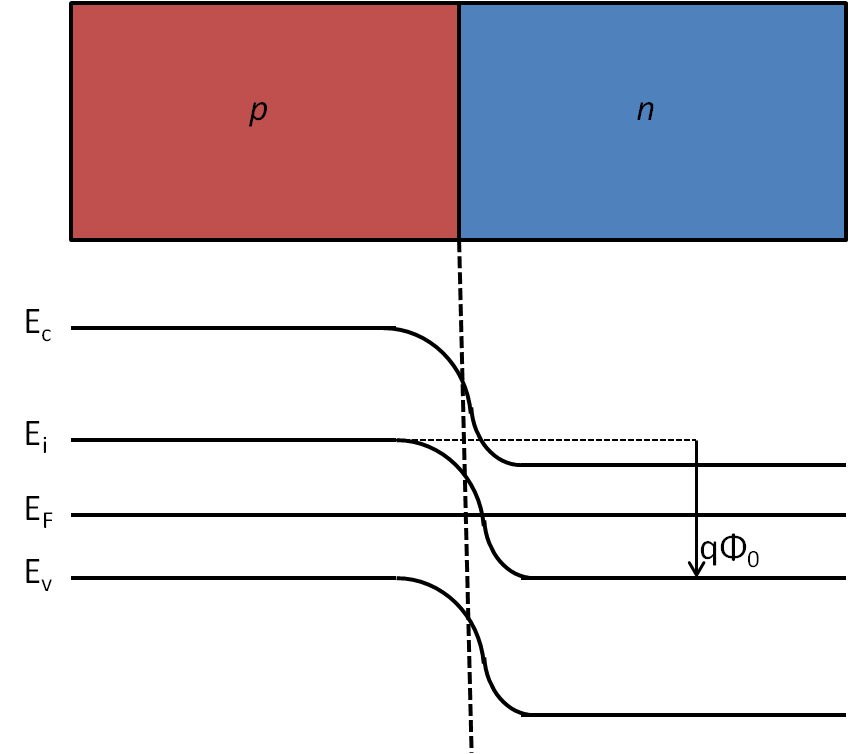
\includegraphics[height=5cm,width=7cm]{figs/unbiased_pn_junction_bands_connected}
    \caption{Energy band diagram of a $p$-$n$ junction.}
\end{figure}

Once the two material types are connected and the Fermi levels are aligned then the electrons
diffuse from the electron-rich $n$-type ($p$-type) material to the electron-lacking (hole-lacking)
$p$-type ($n$-type) region. The diffusion of charges across the junction creates an internal
built-in potential denoted by $\Phi_0$ in fig. \ref{fig:fig02} and in equilibrium is dependent upon 
the thermal voltage ,doping concentrations, and intrinsic carrier concentration of the semiconductor. 
The built-in potential is given by 
\begin{equation}
    \label{eq:phi0_eq}
    \Phi_0 = \frac{k_BT}{q}\ln{\left(\frac{N_aN_d}{n_i^2}\right)},
\end{equation}
where the term $k_BT/q$ is the thermal voltage $V_T$, $N_a$ and $N_d$ are the acceptor and donor doping concentrations, respectively, and
$n_i$ is the intrinsic carrier concentration of the semiconductor. When the electrons (holes) diffuse from the $n$-type ($p$-type) 
region into the $p$-type ($n$-type) region ionized donor (acceptor) atoms are left in their place. This creates a depletion region on each side of the 
junction as shown in fig. 3 where $W_p$ and $W_n$ denotes the depletion region widths on the $p$ and $n$
sides, respectively. 
\begin{figure}[h!]\label{fig:fig03}
    \centering
    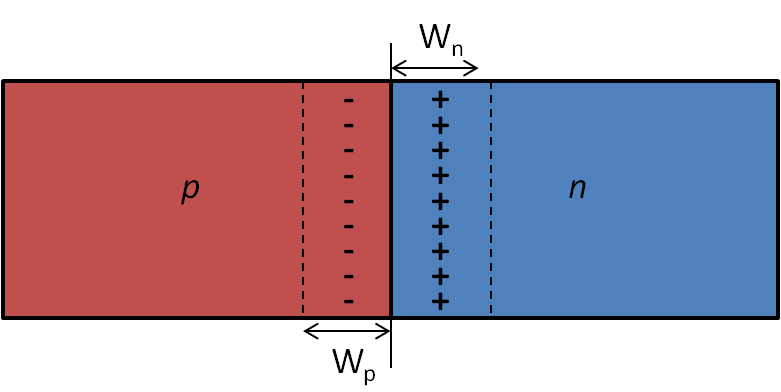
\includegraphics[height=3cm,width=7cm]{figs/unbias_pn_junction_depletion_region}
    \caption{Depletion region width depiction on both the $n$-side and $p$-side, $W_n$ and $W_p$, respectively.}
\end{figure}
In the case of an abrupt $p$-$n$ junction, one that can be modeled as step-function at the transition
from the depletion region to the charge-neutral $p$ and $n$-type regions, there are two boundary conditions that must be 
satisfied. First, that the at the boundary of the depletion region, the electric field must go to zero. Written in 
a mathematical form this implies that 
\begin{equation}
    \label{eq:bc1}
    E(x=W_{p,n}) = 0.
\end{equation}
Second, we define the point $x = 0$ to be the transition within the depletion region from the $p$-type to the $n$-type regions, at this point, the 
electric field must be continuous. This condition written more compactly can be expressed as
\begin{equation}
    \label{eq:bc2}
    E(x = \delta_{p}) = E(x = \delta_{n}),
\end{equation}
where $\delta_p$ and $\delta_n$ are some infinitesimally small distance on the $p$ and $n$-side, respectively. 


%%%%%
\section{$p$-$n$ Junction in Non-Equilibrium}\label{sec:sec003}

\begin{figure}[h!]\label{fig:fig05}
    \centering
    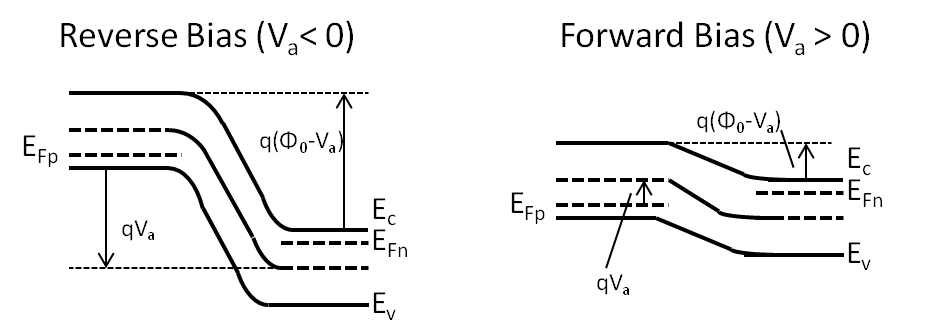
\includegraphics[height=3.5cm,width=8.5cm]{figs/bias_pn_junction}
    \caption{Energy band diagram on $p$-$n$ junction at forward and reverse bias.}
\end{figure}

\begin{figure}[h!]\label{fig:fig07}
    \centering
    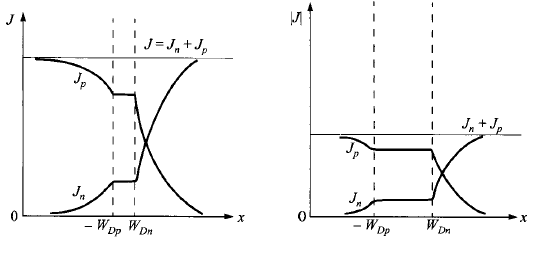
\includegraphics[height=4cm,width=8cm]{figs/schokley_current_reverse_forward}
    \caption{Shockley current density as a function of position within the semiconductor structure at forward and reverse bias.}
\end{figure}

\begin{figure}[h!]\label{fig:fig010}
    \centering
    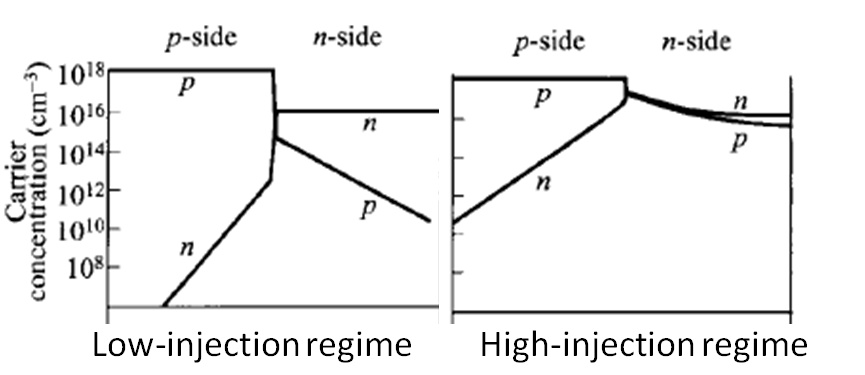
\includegraphics[height=4cm,width=8cm]{figs/high_low_injection}
    \caption{}
\end{figure}

\begin{figure}[h!]\label{fig:fig08}
    \centering
    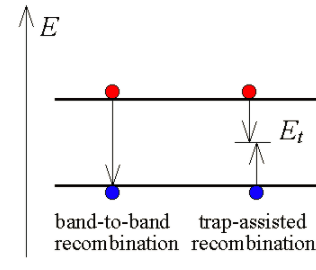
\includegraphics[height=4.5cm,width=5cm]{figs/recomb}
    \caption{Diagram of band-to-band and SRH recombination.}
\end{figure}

\section{$p$-$n$ Junction in $3D$ and Lower-Dimensions}\label{sec:sec004}

\begin{figure}[h!]\label{fig:fig09}
    \centering
    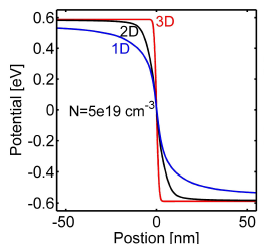
\includegraphics[height=4cm,width=5cm]{figs/2d_3d}
    \caption{Built-in potential as a function of position for $1D$, $2D$, and $3D$.}
\end{figure}

\begin{figure}[h!]\label{fig:fig08}
    \centering
    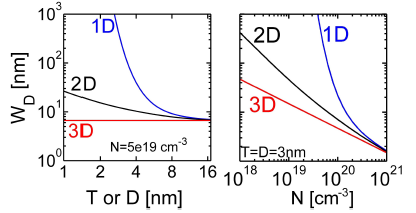
\includegraphics[height=4.5cm,width=8cm]{figs/2d_3d_wd_dep}
    \caption{Depletion width as a function of thickness (left) and carrier concentration (right) for $1D$, $2D$, and $3D$.}
\end{figure}

\section{conclusion}\label{sec:sec005}